\documentclass[]{beamer}

\usepackage{beamerthemesplit}
\usetheme{Madrid}
\usepackage[utf8]{inputenc}
\usepackage[T1]{fontenc}
\usepackage{color}
\usepackage{mathtools}

\usepackage[italian]{babel}
\usepackage{listings}
\usepackage{textcomp}
\usepackage{graphicx}
\usepackage{caption}
\usepackage{eurosym}
\usepackage{float}
\usepackage{epigraph}
\usepackage{amssymb}
\usepackage{pifont}
\usepackage{multirow}


\definecolor{my-green}{RGB}{0,153,0}
\definecolor{my-red}{RGB}{255,0,0}
\setbeamertemplate{itemize items}[default]
\setbeamercolor{block title}{use=structure,fg=blue,bg=white!75!white}
\setbeamercolor{block body}{use=structure,fg=black,bg=white!20!white}
\setbeamersize{text margin left=30pt,text margin right=30pt}
\setbeamertemplate{footline}
{
  \leavevmode%
  \hbox{%
  \begin{beamercolorbox}[wd=.2\paperwidth,ht=2.25ex,dp=1ex,center]{author in head/foot}%
   Luca Vicentini
  \end{beamercolorbox}%
  \begin{beamercolorbox}[wd=.6\paperwidth,ht=2.25ex,dp=1ex,center]{title in head/foot}%
    \usebeamerfont{title in head/foot}\insertshorttitle
  \end{beamercolorbox}%
  \begin{beamercolorbox}[wd=.2\paperwidth,ht=2.25ex,dp=1ex,center]{author in head/foot}%
    \insertframenumber{} / \inserttotalframenumber\hspace*{1ex}
  \end{beamercolorbox}}%
  \vskip0pt%
}

\title{Studio sull'uso di Java \\per la programmazione di una blockchain }
\author{Luca Vicentini - VR408207}
\date{21 marzo 2019}

%*********************************************************************************
% Impostazioni di listings
%*********************************************************************************
\lstset{
	%commentstyle=\color{Green}\ttfamily,
	%keywordstyle=\color{RoyalBlue},%\bfseries,
	%commentstyle=\color{Black}\ttfamily,
	%keywordstyle=\color{Black},%\bfseries,
	language=Java,
	showstringspaces=false,
	columns=flexible,
	basicstyle={\ttfamily\footnotesize},
	frame=l,
	numbers=left,
	numberstyle={\scriptsize},
	%  breaklines=true,
	breakatwhitespace=true,
	tabsize=3,
	inputencoding=utf8,
	extendedchars=true,
	escapechar=■		% ALT+254
}
% file con le impostazioni personali

\begin{document}

\begin{frame}
  \titlepage
  \begin{center}
  	\textbf{Relatore:} Nicola Fausto Spoto
  \end{center}
\end{frame}
\note{Talk for 12 minutes}
                           
%===============================
% INDICE
%===============================
\section{Indice}
%===============================
\begin{frame}{Indice}
	\begin{enumerate}
		\item Bitcoin
			\begin{itemize}
				\item Blockchain
				\item Proof-of-Work
			\end{itemize}
		\item Ethereum
			\begin{itemize}
				\item Smart contract turing-completi e il concetto di \textit{gas}
				\item Ethereum Virtual Machine e Solidity
			\end{itemize}
		\item Takamaka
			\begin{itemize}
				\item Java Virtual Machine
				\item Metodi Java \textit{white-listed}
			\end{itemize}
		\item Individuare metodi Java non deterministici
			\begin{itemize}
				\item java.lang: Object, System
				\item java.util: HashSet, HashMap, Stream, Random
			\end{itemize}
	\end{enumerate}
\end{frame}

%===============================

\begin{frame}{Bitcoin (1/2)}
	
	\begin{columns}[c]
		\column{.7\textwidth} 
			\begin{itemize}
				\item Tecnologia \textbf{peer-to-peer} che non fa uso di un'autorità centrale.
				\item L'emissione di nuova valuta e la gestione delle transazioni viene effettuata collettivamente dalle rete.
			\end{itemize}
		\column{.3\textwidth}
			
\includegraphics[height=3cm]{img/bitcoin-img.png}
	\end{columns}

	\vspace{0.5cm}

	\begin{columns}[c]
		\column{.4\textwidth} 
			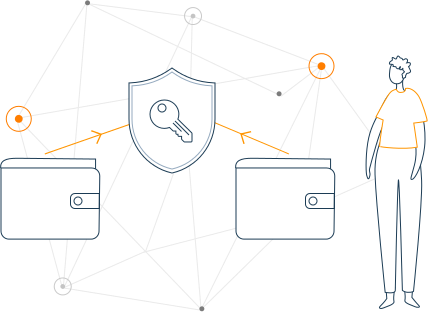
\includegraphics[height=3cm]{img/private-keys.png}
		\column{.6\textwidth}
			Ogni utente crea un \textbf{indirizzo BTC} che utilizzerà per effettuare/ricevere pagamenti che vengono registrati in \textbf{transazioni}.
	\end{columns}
\end{frame}

\begin{frame}{Bitcoin (2/2)}
	\begin{block}{Miner e processo di Mining}
		\begin{itemize}
			\item \textbf{Conferma le transazioni} includendole in un blocco.
			\item Tale blocco rispetta delle regole crittografiche molto rigide che impediscono che qualunque blocco precedente venga modificato.
			\item Il blocco verrà aggiunto alla \textbf{blockchain}.
		\end{itemize}
		 
	\end{block}

	\vspace{0.5cm}

	\textbf{Proof-of-Work} è una sfida globale che comporta l'effettuare ripetutamente l'hash dell'header del blocco, variando un numero casuale, fino a trovare una soluzione con un certo pattern.
\end{frame}

%===============================

\begin{frame}{Ethereum (1/2)}
	\begin{columns}[c]
		\column{.6\textwidth} 
		\begin{itemize}
			\item Infrastruttura open-source, globalmente decentralizzata, per eseguire \textbf{Smart Contract}.
			\item Utilizza la blockchain per sincronizzare e memorizzare le modifiche di stato del sistema e la cripto-valuta \textbf{ether}.
		\end{itemize}
		\column{.3\textwidth}
			
\includegraphics[height=2cm]{img/ethereum.png}
	\end{columns}

	\vspace{0.5cm}

	\begin{center}
		Gli smart contract vengono eseguiti all'interno della\\Ethereum Virtual Machine (\textbf{EVM}) e presentano un\\ \textbf{linguaggio turing-completo}.\textbf{}
	\end{center}
\end{frame}

\begin{frame}{Ethereum (2/2)}
	La Turing-completezza del linguaggio obbliga l'EVM a \textbf{limitare l'esecuzione dei contratti} implementando un meccanismo di misurazione delle risorse chiamato \textbf{gas}.
	
	\vspace{0.5cm}
	
	\begin{block}{Solidity}
		Linguaggio di programmazione \textbf{contract-oriented} che compila dei programmi scritti in Solidity nel linguaggio bytecode per l'EVM. 
	\end{block}

	\begin{center}
		Questo linguaggio è tuttora in via di perfezionamento e soffre la mancanza di strumenti d'aiuto al programmatore.
	\end{center}
\end{frame}

%===============================

\begin{frame}{Takamaka: A Java Framework for Smart Contracts}
	
	\begin{center}
		Framework il cui scopo è \textbf{semplificare lo sviluppo} di smart contract sfruttando competenze e strumenti\\già esistenti del mondo $Java$.
	\end{center}
	
	\begin{block}{}
		\begin{itemize}
			\item Takamaka utilizza un sottoinsieme delle librerie $Java$, chiamate \textbf{white-listed}.
			\item Le analisi effettuate mirano a trovare quei metodi che presentano comportamenti non deterministici.
		\end{itemize}
		 
	\end{block}
	\begin{center}
		\textbf{L'esito di uno smart contract dovrà risultare sempre lo stesso dato il contesto della transazione e lo stato della blockchain in quel momento.}
	\end{center}
\end{frame}

\begin{frame}[fragile]
	\frametitle{Analisi della Classe java.lang.Object}
	\begin{block}{}
		\begin{itemize}
			\item \textbf{hashCode()} Restituisce l'hash code dell'oggetto.\\
			Calcolato utilizzando l'indirizzo in memoria di tale oggetto.
			\begin{lstlisting}
	public int foo() {
		return new Object().hashCode();
	}
			\end{lstlisting}
		\end{itemize}
	\end{block}
	\begin{block}{}
		\begin{itemize}
			\item \textbf{toString()} Stringa che rappresenta testualmente l'oggetto.
			
			\lstinline|getClass().getName() +'@'+ Integer.toHexString(hashCode())|
			\begin{lstlisting}
	public String foo() {
		return new Object().toString();
	}
			\end{lstlisting}
		\end{itemize}
	\end{block}
	\begin{center}
		L'esecuzione dei metodi \lstinline|foo()| risulta non deterministica
	\end{center}
\end{frame}

\begin{frame}[fragile]
\frametitle{Analisi della Classe java.util.HashSet e java.util.HashMap}
Non forniscono garanzie sull'ordine di iterazione del \lstinline|Set|/\lstinline|Map|.\\
Non è garantito che tale ordine rimanga costante nel tempo.
\begin{block}{}
	\begin{itemize}
		\item \textbf{iterator()} Restituisce in iteratore sugli elementi del \lstinline|Set|, gli elementi non vengono restituiti con un ordine particolare.
		
		\item \textbf{values()} Ritorna una \lstinline|Collection view| di tutti i valori contenuti all'interno della \lstinline|Map|.
		
		\begin{lstlisting}
	private HashSet h1 = new HashSet();
	private Map<String, String> h2 = new HashMap<>();
	public Iterator getIterator1() {
		return h1.iterator();
	}
	public Iterator getIterator2() {
		return h2.values().iterator();
	}
		\end{lstlisting}
	\end{itemize}
\end{block}
\end{frame}

\begin{frame}[fragile]
\frametitle{Analisi della Classe java.util.Stream (1/3)}
Una \lstinline|Stream| è una sequenza di elementi che supporta operazioni di aggregazione sequenziali e parallele. Introdotte da \lstinline|Java 8|.
\begin{block}{}
	\begin{itemize}
		\item \textbf{findAny()} Restituisce un qualche elemento all'interno della \lstinline|Stream|. Operazione esplicitamente non deterministica.
		
		\begin{lstlisting}[breaklines=true]
	public String foo() {
		List<String> lst = Arrays.asList( ... );
		
		return lst.stream().filter(s -> s.startsWith("J"))
			.findAny().get();
	}
		\end{lstlisting}
	\end{itemize}
\end{block}
\begin{center}
	Utilizzare \lstinline|findFirst()| per avere un risultato deterministico.
\end{center}
\end{frame}

\begin{frame}[fragile]
\frametitle{Analisi della Classe java.util.Stream (2/3)}
\begin{block}{}
	\begin{itemize}
		\item \textbf{forEach(...)} esegue un'azione per ciascun elemento della \lstinline|Stream|. Il comportamento esplicitamente non deterministico.
		
		\begin{lstlisting}[breaklines=true]
	public void foo() {
		List<String> lst = Arrays.asList( ... );
		
		lst.stream().filter(s -> s.startsWith("J"))
			.forEach(e -> System.out.print(e + " "));
	}
		\end{lstlisting}
	\end{itemize}
\end{block}
\begin{center}
	Non siamo riusciti a trovare un esempio di funzionamento anomalo che provi il non determinismo, ma non può voler dire che tale metodo ritorni sempre i risultati aspettati, bensì che \\\textbf{non possiamo contare su di esso}.
\end{center}
\end{frame}

\begin{frame}[fragile]
\frametitle{Analisi della Classe java.util.Stream (3/3)}
\begin{block}{}
	\begin{itemize}
		\item \textbf{forEachOrdered(...)} esegue un'azione per ciascun elemento della \lstinline|Stream| in base all'ordine di incontro, se la \lstinline|Stream| ne ha definito uno.
		
		\begin{lstlisting}[breaklines=true]
	public void foo() {
		List<String> lst = Arrays.asList( ... );
		
		lst.stream().filter(s -> s.startsWith("J"))
			.forEachOrdered(e -> System.out.print(e + " "));
	}
		\end{lstlisting}
	\end{itemize}
\end{block}
\begin{itemize}
	\item La stream deve avere un'ordine definito.
	\item Si devono utilizzare solo collezioni ordinate.
\end{itemize}
\end{frame}

\begin{frame}[fragile]
\frametitle{Analisi della Classe java.lang.System (1/2)}
\begin{block}{}
	\begin{itemize}
		\item \textbf{currentTimeMillis()} ritorna un \lstinline|long|, rappresenta il tempo corrente misurato in millisecondi trascorsi dal 00:00:00 01/01/1970 UTC.
		\begin{lstlisting}[breaklines=true]
	public long getCurrentMillis() {
		return System.currentTimeMillis();
	}
		\end{lstlisting}
	\end{itemize}
\end{block}
\begin{itemize}
	\item Metodo non deterministico
	\item Utilizzato da \lstinline|java.util.Date|, \lstinline|java.time.Clock| e \lstinline|java.util.Time|.
\end{itemize}
\end{frame}

\begin{frame}[fragile]
\frametitle{Analisi della Classe java.lang.System (2/2)}
\begin{block}{}
	\begin{itemize}
		\item \textbf{nanoTime()} ritorna un valore temporale di esecuzione della JVM misurata in nanosecondi.
		\begin{lstlisting}[breaklines=true]
	public long getNanoTime() {
		return System.nanoTime();
	}
		\end{lstlisting}
	\end{itemize}
\end{block}
\begin{itemize}
	\item Metodo non deterministico
	\item Utilizzato per esempio da \lstinline|java.util.Random|.
\end{itemize}
\end{frame}

\begin{frame}[fragile]
\frametitle{Analisi della Classe java.util.Random (1/2)}
Genera una \lstinline|Stream| di numeri pseudocasuali a partire da un seme \lstinline|seed| modificato ad ogni invocazione.
\begin{block}{}
	\begin{itemize}
		\item \textbf{new Random()} setta un valore di \lstinline|seed| distinto per qualsiasi chiamata, diverso ad ogni invocazione.
		\begin{lstlisting}[breaklines=true]
	public int rnd() {
		return new Random().nextInt();
	}
		\end{lstlisting}
	\end{itemize}
\end{block}
\begin{center}
	Il valore di \lstinline|seed| è derivato da \lstinline|System.nanoTime()| e\\\textbf{sarà diverso per ogni JVM}.
\end{center}
\end{frame}

\begin{frame}[fragile]
\frametitle{Analisi della Classe java.util.Random (2/2)}
\begin{block}{}
	\begin{itemize}
		\item \textbf{new Random(int seed)} setta il valore di \lstinline|seed| indicato che influenzerà i valori generati.
		\begin{lstlisting}[breaklines=true]
	public int rnd() {
		return new Random(1993).nextInt();
	}
		\end{lstlisting}
	\end{itemize}
\end{block}
\begin{center}
	\lstinline|58 83 97 81 90 70 41 94 80 79 51 83 32 28 73 ...|
\end{center}
\begin{itemize}
	\item Comportamento deterministico
	\item Restituisce sempre la stessa sequenza
\end{itemize}
\end{frame}

\begin{frame}{In sintesi}
	% Please add the following required packages to your document preamble:
	% \usepackage{multirow}
	\begin{table}[]
		\begin{tabular}{|c|c|c|}
			\hline
			\multirow{2}{*}{java.lang.Object} & hashCode() & \ding{55} \\ \cline{2-3} 
			& toString() & \ding{55} \\ \hline
			java.util.HashSet & iterator() & \ding{55} \\ \hline
			java.util.HashMap & values().iterator() & \ding{55} \\ \hline
			\multirow{5}{*}{java.util.Stream} & findAny() & \ding{55} \\ \cline{2-3} 
			& \textbf{findFirst()}* & \ding{51}  \\ \cline{2-3} 
			& forEach(...) & \ding{55} \\ \cline{2-3} 
			& \textbf{forEachOrdered(...)}* & \ding{51}  \\ \cline{2-3} 
			& peek() & \ding{55} \\ \hline
			\multirow{2}{*}{java.lang.System} & currentTimeMillis() & \ding{55} \\ \cline{2-3} 
			& nanoTime() & \ding{55} \\ \hline
			\multirow{2}{*}{java.util.Random} & Random() & \ding{55} \\ \cline{2-3} 
			& Random(int seed) & \ding{51} \\ \hline
		\end{tabular}
	\end{table}
\begin{center}
	\ding{55} metodi per la concorrenza e \lstinline|parallelStream()|.
\end{center}
\end{frame}

\begin{frame}
\begin{center}
	Fine\\
	Grazie per l'attenzione
\end{center}
\end{frame}

\end{document}
